\documentclass{article}
\usepackage{tikz}
\usetikzlibrary{arrows.meta}

\begin{document}

\begin{figure}[h]
    \centering
    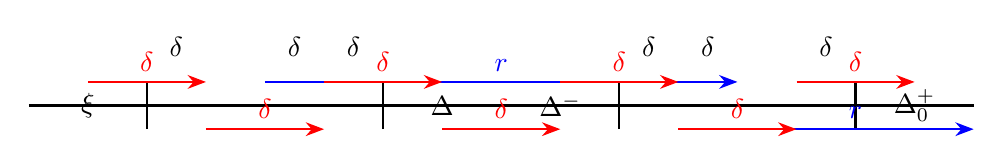
\begin{tikzpicture}[scale=1.5]
        % Draw the horizontal line
        \draw[thick] (-4,0) -- (4,0);
        
        % Draw the vertical lines
        \draw[thick] (-3,-0.2) -- (-3,0.2);
        \draw[thick] (-1,-0.2) -- (-1,0.2);
        \draw[thick] (1,-0.2) -- (1,0.2);
        \draw[thick] (3,-0.2) -- (3,0.2);
        
        % Draw the labels for the vertical lines
        \node at (-3.5,0) {$\xi$};
        \node at (-0.5,0) {$\Delta$};
        \node at (0.5,0) {$\Delta^-$};
        \node at (3.5,0) {$\Delta_0^+$};
        
        % Draw the blue arrows
        \draw[blue, thick, -Stealth] (-2,0.2) -- node[midway, above] {$r$} (2,0.2);
        \draw[blue, thick, -Stealth] (2,-0.2) -- node[midway, above] {$r$} (4,-0.2);
        
        % Draw the red arrows
        \draw[red, thick, -Stealth] (-3.5,0.2) -- node[midway, above] {$\delta$} (-2.5,0.2);
        \draw[red, thick, -Stealth] (-2.5,-0.2) -- node[midway, above] {$\delta$} (-1.5,-0.2);
        \draw[red, thick, -Stealth] (-1.5,0.2) -- node[midway, above] {$\delta$} (-0.5,0.2);
        \draw[red, thick, -Stealth] (-0.5,-0.2) -- node[midway, above] {$\delta$} (0.5,-0.2);
        \draw[red, thick, -Stealth] (0.5,0.2) -- node[midway, above] {$\delta$} (1.5,0.2);
        \draw[red, thick, -Stealth] (1.5,-0.2) -- node[midway, above] {$\delta$} (2.5,-0.2);
        \draw[red, thick, -Stealth] (2.5,0.2) -- node[midway, above] {$\delta$} (3.5,0.2);
        
        % Draw the labels for the blue arrows
        \node at (-1.75,0.5) {$\delta$};
        \node at (1.75,0.5) {$\delta$};
        
        % Draw the labels for the red arrows
        \node at (-2.75,0.5) {$\delta$};
        \node at (-1.25,0.5) {$\delta$};
        \node at (1.25,0.5) {$\delta$};
        \node at (2.75,0.5) {$\delta$};
    \end{tikzpicture}
    \caption{Schematic picture of $\Delta, \Delta^-, \Delta_0, \Delta^+$. We will usually take $r = \frac{\tau}{2n}$ and $\delta = \frac{1}{2m}$ for $n \ll m$, for example, later in the paper we use $m = n^{1+\beta'}$ below.}
    \label{fig:delta_schematic}
\end{figure}

\end{document}